% *************************
% **     ANTECEDENTES    **
% *************************

\section{Antecedentes}
% Apellido letra del Nombre (Juan Perez), año, titulo del trabajo, institucion, pais
\noindent
Perez J, (2013),\textit{Nombre del proyecto}, Institución donde se desarrollo, País.\\

\noindent
\textbf{Conclusiones:}
\begin{itemize}
	\item Conclusión 1.
	\item Conclusión 2.
	\item Conclusión N.
\end{itemize}

\noindent
\textbf{Comentario:} Aquí se expone de que manera nos servirá este proyecto, si es para continuar la investigación, sacar marco teórico, o algún algoritmo o pruebas consideradas útiles para nuestro trabajo futuro.\\

\noindent
Benitez J, (2021),\textit{cuando las computadoras sienten}, Universidad de distrital Guadalajara, Mexico.\\

\noindent
\textbf{Conclusiones:}
\begin{itemize}
	\item Conclusión 1.
	\item Conclusión 2.
	\item Conclusión N.
\end{itemize}

\noindent
\textbf{Comentario:} Aquí se expone de que manera nos servirá este proyecto, si es para continuar la investigación, sacar marco teórico, o algún algoritmo o pruebas consideradas útiles para nuestro trabajo futuro.


% *************************
% **     MARCO TEÓRICO   **
% *************************
\section{Marco Teórico}
\subsection{Sobre el tema uno}
Hablamos un poco sobre el tema en cuestión como para que el lector se entere de que va el trabajo a desarrollar y nunca olvidar las referencia de donde las sacamos, pueden ser libros físico o libros electrónicos como también contenido de paginas web, o papers \citep{Larranaga}.


\subsection{Sobre el tema dos}
Hablamos un poco sobre el tema en cuestión como para que el lector se entere de que va el trabajo a desarrollar y nunca olvidar las referencia de donde las sacamos, pueden ser libros físico o libros electrónicos como también contenido de paginas web, o papers\citep{herz01}.
\subsubsection{Algún tema mas}
Esto si por allí queremos dar mas énfasis a algún tema pero no hay indentado esto queda solo allí, y ojo  ver Figura \ref{fig:ojo}, todo con sus referencia bibliográficas estilo APA

\begin{figure}[!ht]
\caption{Ojo Digital}
    \begin{center}
    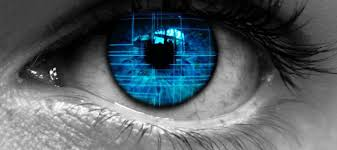
\includegraphics[scale=0.5]{imagenes/ojo.jpg}\\    
    \end{center}
    \label{fig:ojo}
    \textit{Nota.} Solo si NO es elaboración propia.
\end{figure}

\subsection{Sobre el tema tres}
Hablamos un poco ver (Tabla~\ref{tab:contenido}) sobre el tema en cuestión como para que el lector se entere de que va el trabajo a desarrollar y nunca olvidar las referencia de donde las sacamos, pueden ser libros físico o libros electrónicos como también contenido de paginas web, o papers vistos en la Tabla~\ref{tab:resultados}.

\begin{table}[!ht]
\centering
\begin{threeparttable}
    \caption{Descripción del contenido}
    \label{tab:contenido}
    \begin{tabular}{@{}lllll@{}}
        \toprule
        COD  & DESCRIPCIÓN   & CR & HRS & CAT \\ 
        \midrule
        A123 & Matemática 01 & 2  & 4   & OE  \\
        A321 & Algorítmica   & 5  & 4   & OE  \\
        A456 & Ensamblador   & 2  & 2   & EE  \\ 
        \bottomrule
    \end{tabular}
    \begin{tablenotes}
        \item \textit{Nota.} Solo si NO es elaboración propia.
    \end{tablenotes}
\end{threeparttable}
\end{table}

\begin{table}[ht]
\centering
\begin{threeparttable}
    \caption{Promedios de calificaciones por grupo}
    \label{tab:resultados}
    \begin{tabular}{lccc}
        \toprule
        \textbf{Grupo} & \textbf{N} & \textbf{Media} & \textbf{Desviación estándar} \\
        \midrule
        A & 25 & 14.8 & 1.25 \\
        B & 27 & 15.2 & 1.18 \\
        C & 26 & 13.9 & 1.40 \\
        \bottomrule
    \end{tabular}
    \begin{tablenotes}
    \small
    \item Nota. N = número de participantes.
    \end{tablenotes}
\end{threeparttable}
\end{table}

\subsection{Sobre el tema cuatro}
Hablamos un poco sobre el tema en cuestión como para que el lector se entere de que va el trabajo a desarrollar ver Figura~\ref{fig:masOjos} y nunca olvidar las referencia de donde las sacamos, pueden ser libros físico o libros electrónicos como también contenido de paginas web, o papers \cite{wikiRed}.

\begin{figure}[!ht]
\caption{Resultado de ver con otro ojo.}
    \begin{center}
    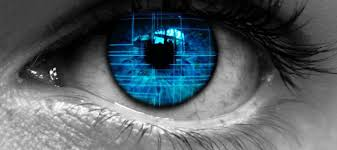
\includegraphics[scale=0.5]{imagenes/ojo.jpg}\\    
    \end{center}
    \label{fig:masOjos}
    \textit{Nota.} Solo si NO es elaboración propia.
\end{figure}

% *************************
% **     METODOLOGIA     **
% *************************

\section{Metodología}

\subsection{Enfoque}
Aquí hay que elegir cuidadosamente el enfoque que tiene la investigación según un único autor para no estar construyendo un método de investigación mezclado, recomiendo usar a \citep{sampieri} , quien enfoca los trabajos de investigación en \textbf{Cualitativos, \textcolor{blue}{Cuantitativos}  o Mixtos}.

\subsection{Alcance}
\paragraph{Explorativa}: Identifican y organizan temas nuevos en un campo de aplicación poco estudiado. 
\paragraph{\textcolor{blue}{Descriptiva}}: En este alcance sí se miden variables, pero de forma individual. Su objetivo no es vincularlas (correlación) ni determinar su causa (explicación), sino cuantificar la presencia o magnitud de cada variable en la población. Por ejemplo: medir la frecuencia de uso de un sistema (Variable 1) y el nivel de satisfacción del usuario (Variable 2), pero sin buscar la relación entre ambas.
\paragraph{Correlacional}: Analizan la relación entre variables tal como ocurren en el mundo real, sin manipulación experimental.
\paragraph{Explicativa}: Manipulan deliberadamente variables independientes para analizar su efecto sobre variables dependientes y explicar causalmente el fenómeno estudiado.

Las dos primeras no necesitan de Hipótesis y por ende son las mas recomendadas mientras que las 2 ultimas requieren de Hipótesis y un análisis de variables eso no quiere decir que sean difíciles solo hay que tener mas tiempo.
Para el caso de las correlacionales sus variables serán de observación mientras que para las explicativas sus variables serán dependientes e independientes.

Para cada variable en su matriz de operacionalizacion debemos de considerar: 
\begin{itemize}
    \item Variable: Aspecto que se quiere medir o analizar. Puede ser dependiente (efecto) o independiente (causa) u observable.
    \item Dimensión: Componentes o aspectos específicos de una variable compleja.
    \item Indicador: Forma concreta de medir cada dimensión (pregunta, ítem, observable).
\end{itemize}

\subsection{Diseño}
Un estudio \textbf{exploratorio} o \textbf{descriptivo} necesita una estrategia sobre cuándo y dónde recolectar los datos. El diseño \textcolor{blue}{No Experimental Transversal} es la respuesta, ya que establece que la recolección se hará en un único punto en el tiempo y en el contexto natural (sin manipulación), lo cual es ideal para describir o explorar.

% *************************
% **     HIPOTESIS      **
% *************************
\subsection{Hipótesis}
(\textcolor{red}{opcional}) Según alcance de la investigación seleccionado.\\

Los trabajos cuantitativos consideran los alcances:
\begin{itemize}
	\item Explorativa: \textbf{NO} tiene hipótesis.
	\item Descriptiva: \textbf{NO} tiene hipótesis.
	\item Correlacional: \textbf{SI} tiene hipótesis, tiene estudio de variables, análisis de resultados y discusión.
	\item Explicativa: \textbf{SI} tiene hipótesis, tiene manipulación de variables independientes, análisis de resultados y discusión.
\end{itemize}

\subsection{Población y muestra}
A esta altura hay que aclara que la escuela no lo menciona pero son puntos a considerar opcionales pero recomendados desde mi punto de vista.

Considerar la \textbf{población y muestra}: que serían los usuarios finales de sistemas de información para medir niveles de satisfacción, la cantidad de elementos en un data set para trabajo de IA, o el nro de procesos afectados si es manejo de ISO`s por ejemplo.

Tambien colocar previo a este punto una \textbf{tabla de operacionaliación de variables} medibles en el caso de descriptivas pero individuales. 

\subsection{Metodología de desarrollo}
Uso de alguna metodología para el desarrollo del sistema ejemplo (RUP, SCRUM...) o bigdata(crisp database), Design Science Research (DSR) para IA, etc.